\chapter{Mid-Price Prediction and Simulation Using Hawkes Processes}

Following the analysis of Generative Adversarial Networks, we now explore point processes for mid-price prediction. This chapter models the limit order book using a calibrated Hawkes process. We simulate order arrivals and evolve the order book state to predict the mid-price path.

\section{Problem Setup and Event Classification}

We use historical message and order book data to calibrate our model. We extract a subset of 20,000 consecutive market events. The timestamps are normalized to start at zero.

We classify the order flow into a 6-dimensional system. This classification depends on the order type and trade direction. The six event streams are:
\begin{itemize}
    \item Buy Market Orders (Executions)
    \item Sell Market Orders
    \item Buy Limit Orders (Submissions)
    \item Sell Limit Orders
    \item Cancel Bids
    \item Cancel Asks
\end{itemize}

\section{Hawkes Process Calibration}

We model the arrivals of these six events using a mutually exciting Hawkes process. We choose an exponential decay kernel with a fixed decay parameter ($\beta = 1.5$).

We estimate the model parameters using Maximum Likelihood Estimation. We calculate the log-likelihood over the empirical event streams. We minimize the negative log-likelihood using the L-BFGS-B optimization algorithm. This provides the baseline intensities ($\mu$) and the 6x6 excitation matrix ($\alpha$).

A key requirement is process stability. The Hawkes process is only stable if the spectral radius of the excitation matrix is strictly less than one. We enforce this constraint by calculating the eigenvalues and capping the maximum eigenvalue of the calibrated excitation matrix.

\section{Order Book Simulation Algorithm}

We simulate the arrival of future events using a standard thinning algorithm. The simulation runs up to a defined time horizon ($T = 100$).

We use these simulated events to evolve the state of the limit order book. We initialize the simulation using the real market bid price, ask price, and top-of-book queue sizes. The queues then update dynamically based on the simulated event types:
\begin{itemize}
    \item Market orders decrease the opposite side queue.
    \item Limit orders increase the same side queue.
    \item Cancel orders decrease the same side queue.
\end{itemize}

A price change is triggered when a queue size drops to zero or below. The best price shifts by one tick. The depleted queue is then replenished. We determine the new queue size by randomly sampling from the empirical distribution of real market queues. Finally, we add a small amount of Gaussian noise to the calculated mid-price to reflect market micro-variations.

\section{Simulation Results}

We evaluate the simulator by comparing the generated synthetic data against the real market data.

\subsection{Inter-arrival Times}
We plot the distribution of time differences between consecutive events. The simulated inter-arrival times closely follow the real empirical distribution. The Hawkes process successfully captures the timing dynamics of the market.

\begin{figure}[h]
    \centering
    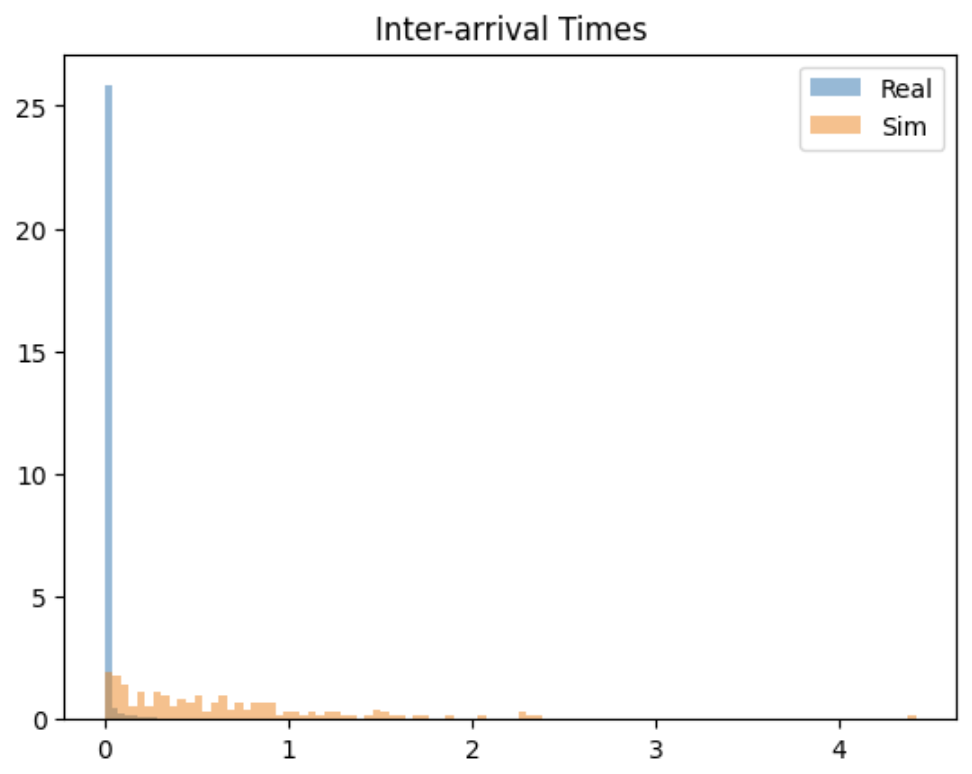
\includegraphics[width=0.82\linewidth]{Hawkes Inter Arrival.png}
    \caption{\textit{Inter-arrival Times Distribution: Real vs. Simulated}}
    \label{fig:interarrival}
\end{figure}

\subsection{Return Distribution and Volatility}
We calculate the price returns from the mid-price paths. The model struggles to perfectly match the empirical volatility. The real market volatility is calculated at roughly $0.0013$. The simulated volatility is significantly higher at roughly $0.0125$.

\begin{figure}[h]
    \centering
    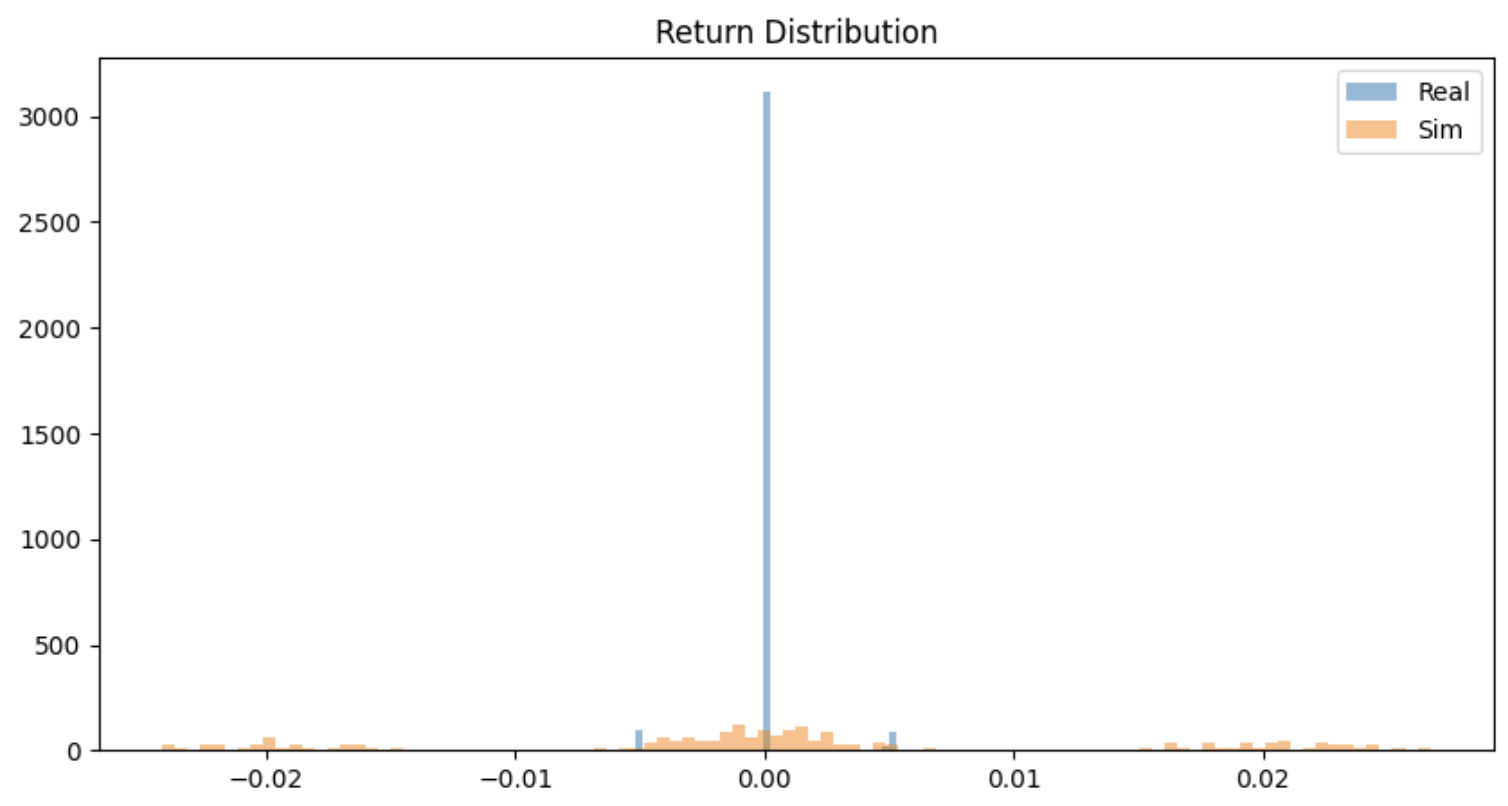
\includegraphics[width=0.82\linewidth]{Hawkes Return Distribution.png}
    \caption{\textit{Return Distribution: Real vs. Simulated}}
    \label{fig:returndist}
\end{figure}

\subsection{Price Path Trajectory}
The simulated price path captures the general microscopic movement but exhibits a wider overall range. The real mid-price ranges between 30.96 and 31.07. The simulated mid-price stretches from 30.93 to 31.15. The overestimation of volatility directly causes this expanded price range.

\begin{figure}[h]
    \centering
    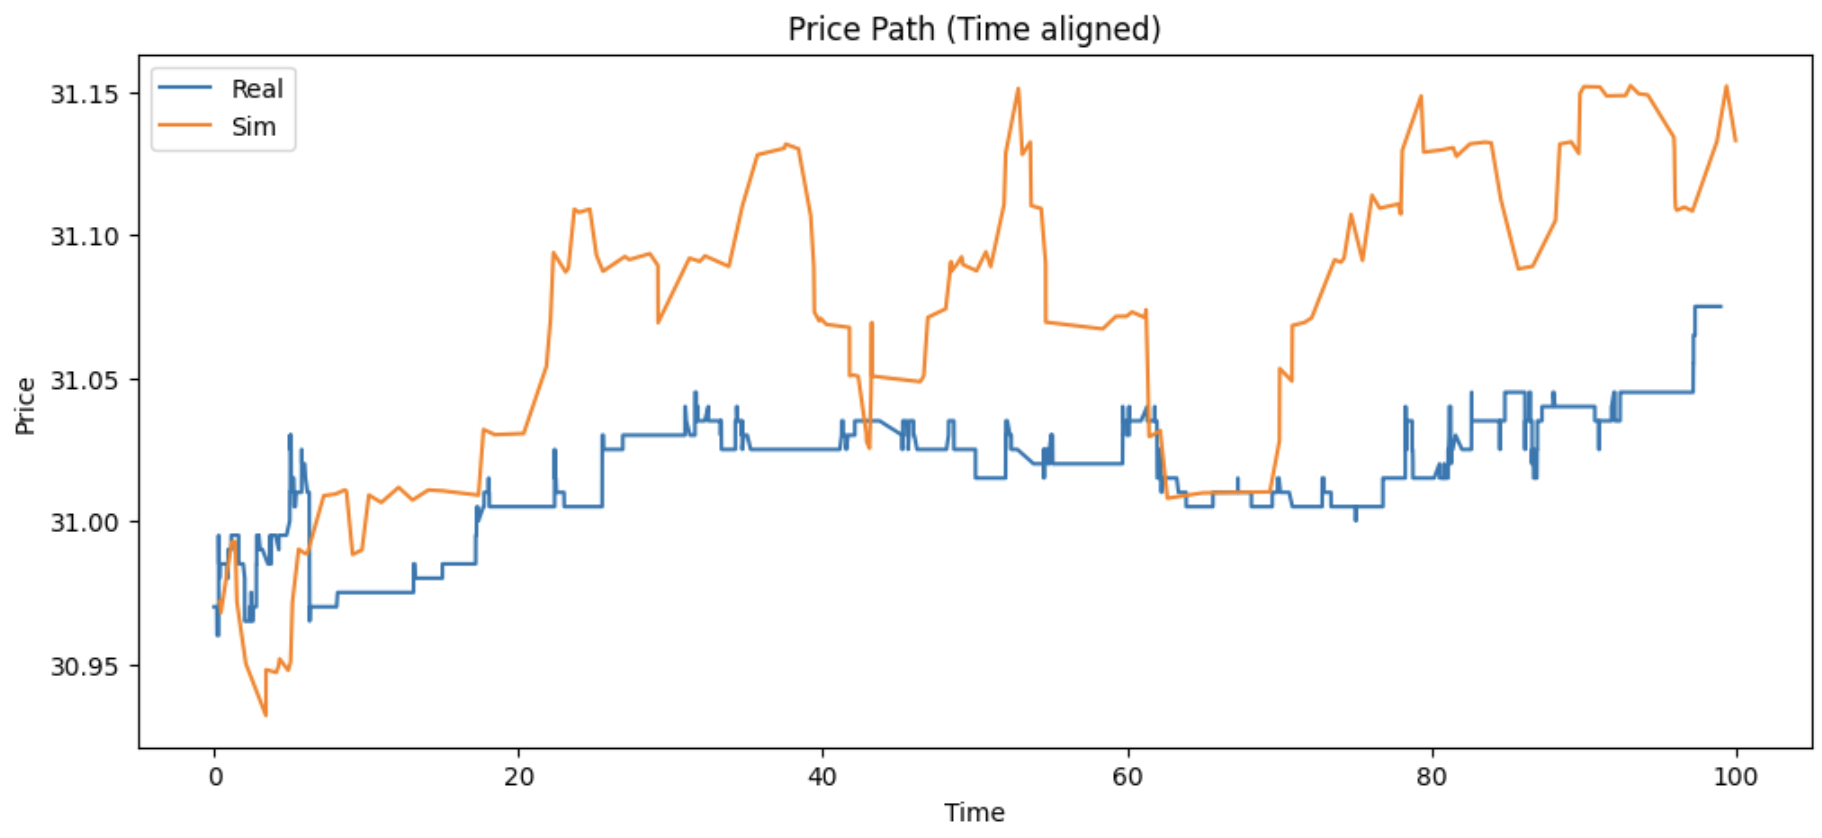
\includegraphics[width=0.82\linewidth]{Hawkes Price Path.png}
    \caption{\textit{Price Path Comparison over Time}}
    \label{fig:pricepath}
\end{figure}

\section{Conclusion}

A 6-dimensional Hawkes process effectively models the self-exciting nature of order flow. It generates highly accurate event arrival times. However, this specific simulation framework overestimates mid-price volatility. Simulating realistic price paths requires more complex handling of order sizes and queue replenishment mechanics.